\documentclass[10.5pt
%,draft
]{article}

\usepackage{ctex}
\usepackage{graphicx}
\usepackage{amsmath}
\usepackage{xcolor}
\usepackage{physics}
\usepackage{geometry}
\usepackage{natbib}
\usepackage{subcaption}

\renewcommand{\refname}{参考文献}
\renewcommand{\figurename}{图}
\renewcommand{\abstractname}{摘要}

\def\due{2023 年 4 月 7 日周五 8:40}
\def\Term{2023 年春季}
\def\Course{磁流体力学的数值模拟方法}

\begin{document}

\title{行波方程和 Burgers 方程的数值计算 \\
  第 2 次作业\footnote{\Term\Course}}

\author{徐均益\footnote{ID: SA22168021 Email: jyxu@mail.ustc.edu.cn}
  \and
  余航\footnote{ID: SA22168021 Email: yh131996@mail.ustc.edu.cn}
  \and
  陈宇韬\footnote{ID: SA22214014 Email: chenyut@mail.ustc.edu.cn}
}

\date{%
\scriptsize%
%CAS Key Laboratory for Basic Plasma Physics, School of Earth and Space Sciences,
%\\
%University of Science and Technology of China, Hefei, Anhui 230026, China
中国科学技术大学地球与空间科学学院, 合肥 230026
中国科学技术大学物质科学研究院等离子所, 合肥 230026
%
}


\maketitle

\begin{abstract}
课程《磁流体力学的数值模拟方法》的第二次作业,讨论一维单一变量双曲型方程,其中包括行波方程和 \textit{Burgers} 方程的有限差分数值解法,
结合分析讨论几种常用的差分格式的特点. 如 \textit{Upwind} 格式, \textit{Lax-Wendroff} 格式,斜率补偿的限制器模式。行波方程与 \textit{Burgers} 方程采用了两种不同的初始输入,其中行波方程主要讨论在传播同样的距离条件下不同方法的耗散程度;而 \textit{Burgers} 方程则采用行波方程中比较好的斜率补偿限制器的方法,对波形在传播的不同时刻进行观测,同时与理论值进行对比分析结果。
\end{abstract}

\section{引言与背景}
波动是流体运动的一种重要形式,一般指的是在一个已经处于平衡态的流体体系中,收到小扰动时,其对应物理量的扰动随着时间在空间上进行传播,其在时间上与空间上具有双重周期性。其中对于线性一维的波动方程
\begin{align}
\frac{\partial^2 u}{\partial t^2} - a^2 \frac{\partial^2 u}{\partial x^2} = 0
\label{EqnCon}
\end{align}
可以变形分解为两个方向的行波解。
\begin{align}
\left( \frac{\partial }{\partial t} + a \frac{\partial }{\partial x} \right) \left( \frac{\partial }{\partial t} - a \frac{\partial }{\partial x} \right) u= 0
\end{align}
本次研究对象为其中正向传播的行波方程。

另外流体力学中也会存在一些典型的非线性波动现象,如激波等等。在激波发生时,会在上游流体与下有流体之间出现一层流体状态量急剧空间变化的过程。为了模拟激波的生成,我们采用了简单的非线性 \textit{Burgers} 方程
\begin{align}
\frac{\partial u}{\partial t} + u \frac{\partial u}{\partial x} = 0, \label{EqnBurgers}
\end{align}
通过选用具体的某些初始函数的形状,通过模拟实验观察激波的生成。

本次实验主要以上述两个波动方程为基础,通过对比不同的模拟数值方法与参数,来分析对比不同的数值方法的特点与优劣,其中包括 \textit{Upwind} 格式, \textit{Lax-Wendroff} 高精度格式,以及采用斜率修正的限制器格式。

\section{实验方法以及对应的理论部分}
数值实验总体思路:采用适当的空间间隔将一维空间网格化,然后设计具体的数值物理量的网格值内容,在将时间网格与空间网格的比$C = \Delta t / \Delta x$作为可调节参数,使用程序进行迭代更新网格内容。
方程包括行波方程与 \textit{Burgers} 方程两种。方法主要是以 \textit{Upwind} 格式探讨不同的$C$对于稳定性的影响,然后固定某一个$C$下讨论不同格式的数值方法对于稳定性的影响。

其中具体的方程以及不同的数值方法的表达式形式如下

\subsection{行波方程}
\begin{align}
\frac{\partial u}{\partial t} + \frac{\partial u}{\partial x} = 0
\end{align}

行波方程对应的 \textit{Upwind} 格式\cite{he_volume-preserving_2015}
\begin{equation}
u_j^{n+1} = u^n - \frac{\Delta t}{\Delta x} (u_j^n - u_{j-1}^n), \label{EqnUpwind}
\end{equation}

行波方程对应的 \textit{Lax-Wendroff} 格式
\begin{align}
	u_j^{n+1} 
	=&
	u_j^{n} 
	-
	\frac{a \Delta t}{ 2 \Delta x } (  	u_{j+1}^{n} - u_{j-1}^{n} ) \\
	&+ \frac{1}{2} \left( \frac{a \Delta t}{ \Delta x } \right)^2 (  	u_{j+1}^{n}- 2 u_j^n + u_{j-1}^{n} ),
\end{align}

 
行波方程对应的\textit{Minmod} 限制器格式
\begin{equation}
\begin{aligned}
u_i^{n+1}= & \frac{a \Delta t}{\Delta x}\left(u_{i-1}^n+\frac{1}{2}(\Delta x-a \Delta t) \sigma_{i-1}^n\right)+ \\
& \left(1-\frac{a \Delta t}{\Delta x}\right)\left(u_i^n-\frac{1}{2} a \Delta t \sigma_i^n\right) \\
= & u_i^n-\frac{a \Delta t}{\Delta x}\left(u_i^n-u_{i-1}^n\right)-\frac{1}{2} \frac{a \Delta t}{\Delta x}(\Delta x-a \Delta t)\left(\sigma_i^n-\sigma_{i-1}^n\right),
\end{aligned}
\end{equation}
其中
\begin{equation}
	\sigma_i^n = \verb|Minmod| ( \frac{u_i^n - u_{i-1}^{n}}{ \Delta x }, \frac{u_{i+1}^n - u_{i}^{n}}{ \Delta x } )
\end{equation}
及
\begin{equation}
	\verb|Minmod|(a, b) = 
	\begin{cases}
		a, \qif |a| < |b| \qand ab > 0\\
		b, \qif |a| > |b| \qand ab > 0\\
		0, \qif ab \leq 0.
	\end{cases}
\end{equation}

\subsection{\textit{Burgers} 方程}

\begin{align}
\frac{\partial u}{\partial t} + u \frac{\partial u}{\partial x} = 0
\end{align}

\textit{Burgers} 方程对应的 \textit{Upwind} 格式
\begin{equation}
u_j^{n+1} = u^n - \frac{\Delta t}{\Delta x} \left( \frac{1}{2} (u_j^n)^2 - \frac{1}{2} (u_{j-1}^n)^2\right)
\end{equation}

\textit{Burgers} 方程对应的 \textit{Minmod} 限制器格式
\begin{equation}
\begin{aligned}
u_i^{n+1}=&
  u_i^n-\frac{a \Delta t}{\Delta x}\left( \frac{1}{2} (u_i^n)^2- \frac{1}{2} (u_{i-1}^n)^2 \right)-
 &\frac{1}{2} \frac{a \Delta t}{\Delta x}(\Delta x-a \Delta t)\left(\sigma_i^n-\sigma_{i-1}^n\right)
\end{aligned}
\end{equation}
其中
\begin{equation}
	\sigma_i^n = \verb|Minmod| \left( \frac{ \frac{1}{2} (u_i^n)^2 - \frac{1}{2} (u_{i-1}^{n})^2 }{ \Delta x }, \frac{ \frac{1}{2} (u_{i+1}^n)^2 - \frac{1}{2} (u_{i}^{n})^2}{ \Delta x } \right)
\end{equation}
\begin{equation}
	\verb|Minmod|(a, b) = 
	\begin{cases}
		a, \qif |a| < |b| \qand ab > 0\\
		b, \qif |a| > |b| \qand ab > 0\\
		0, \qif ab \leq 0.
	\end{cases}
\end{equation}


\section{实验结果及解释描述}
\subsection{行波方程数值模拟部分}
考察方程
\begin{align}
\frac{\partial u}{\partial t} + \frac{\partial u}{\partial x} = 0
\end{align}
在初值条件
\begin{align}
& u|_{t=0} = \left\{\begin{array}{ll} 0.0, & x < -0.4, \\
1.0 - |x + 0.3| / 0.1, & -0.4 \le x < -0.2, \\
0.0, & -0.2 \le x < -0.1, \\
1.0 , & -0.1 \le x < 0.0, \\
0.0, & x \ge 0.0
\end{array}\right.
\end{align}
下分别设计几组不同的参数与不同的数值方法,其中模拟结果如图~\ref{LinearW}

\begin{figure} 
\centering
\begin{subfigure}{.48\linewidth}
	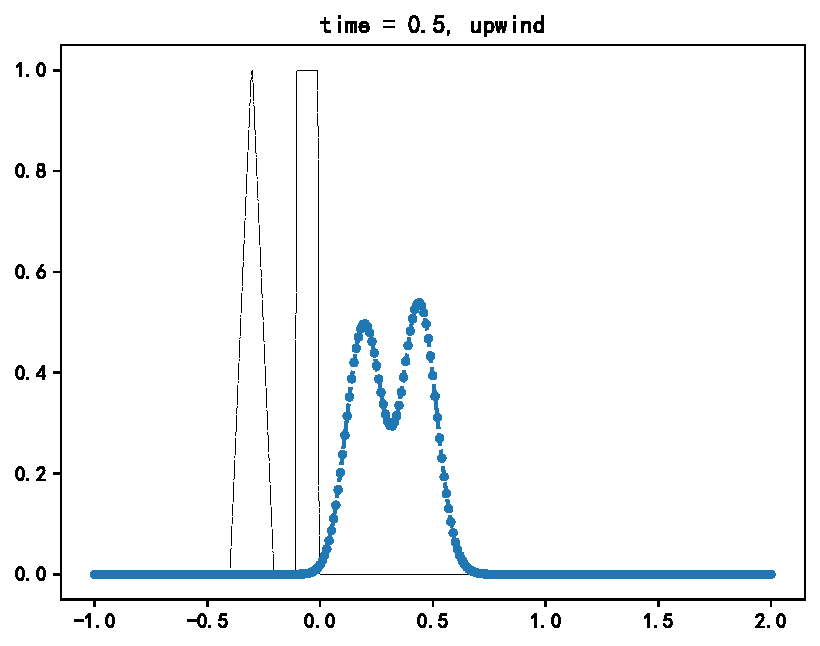
\includegraphics[width=\textwidth]{figures/problem1_upwind0.05.pdf}
  \caption{}
  \label{fig:problem1-1}
\end{subfigure}
\hfill
\begin{subfigure}{.48\linewidth}
  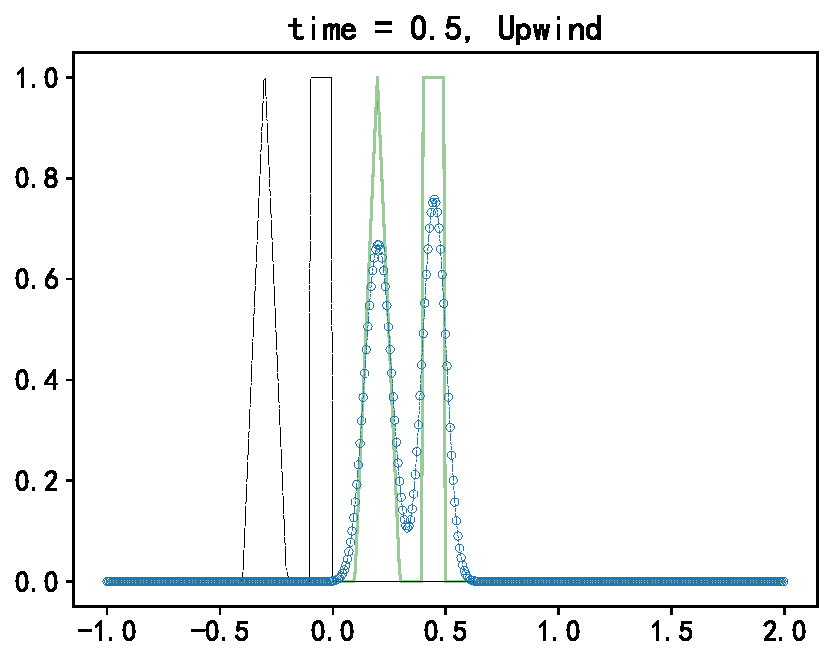
\includegraphics[width=\textwidth]{figures/problem1_upwind0.5.pdf} % second figure itself
  \caption{}
  \label{fig:problem1-2}
\end{subfigure}
\begin{subfigure}{.48\linewidth}
  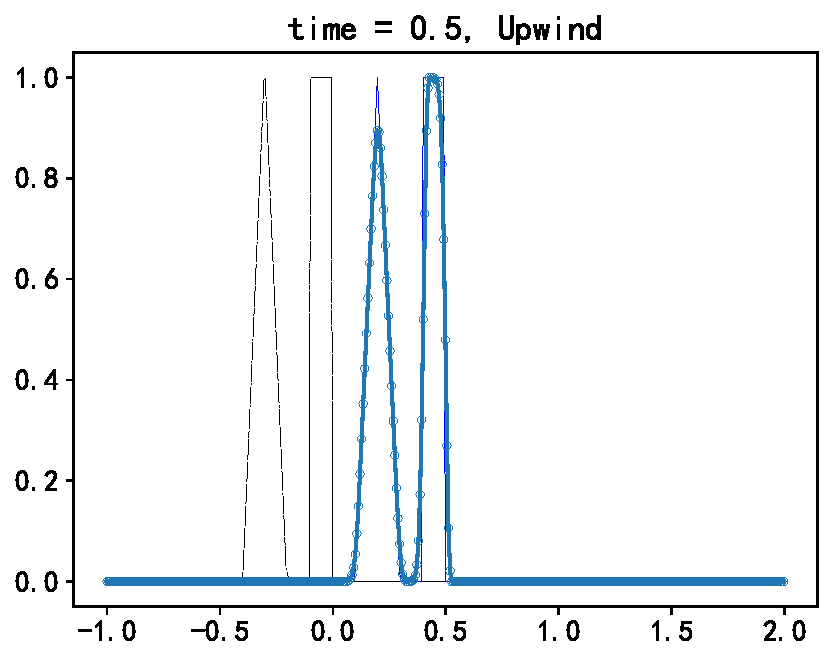
\includegraphics[width=\textwidth]{figures/problem1_upwind0.95.pdf}
  \caption{}
  \label{fig:problem1-3}
\end{subfigure}
\hfill
\begin{subfigure}{.48\linewidth}
  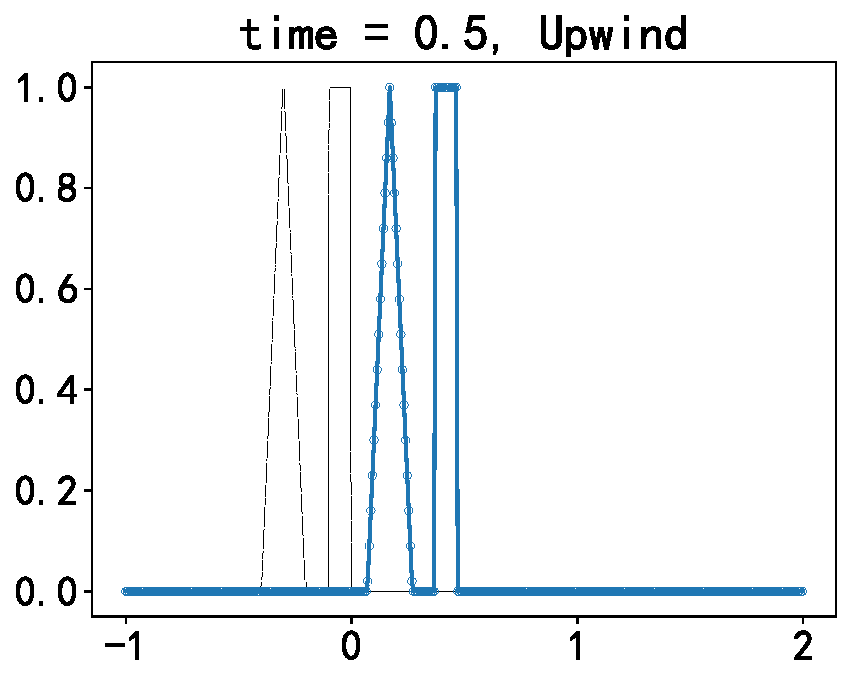
\includegraphics[width=\textwidth]{figures/problem1_upwind1.0.pdf}
  \caption{}
  \label{fig:problem1-4}
\end{subfigure}
\begin{subfigure}{.48\linewidth}
  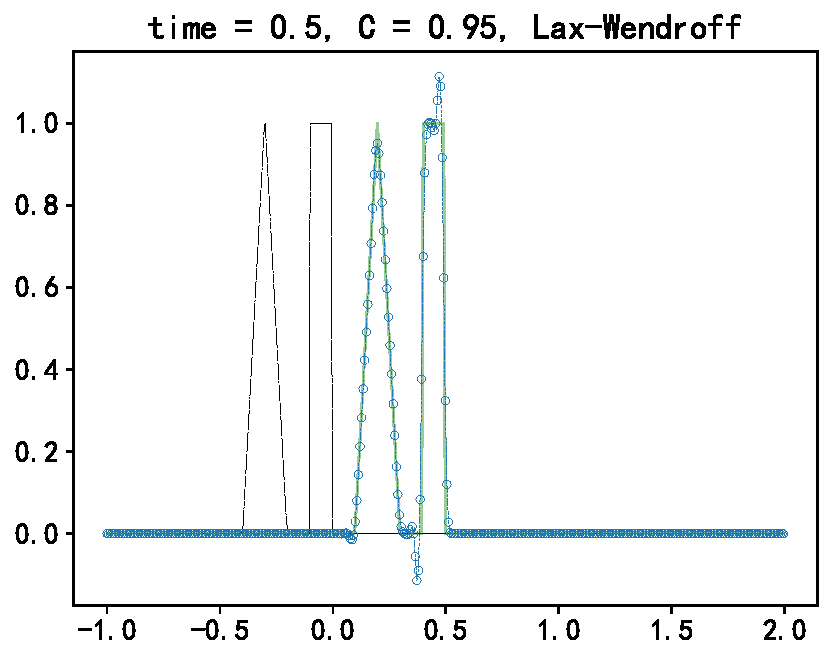
\includegraphics[width=\textwidth]{figures/problem1_lax_wendroff0.95.pdf}
  \caption{}
  \label{fig:problem1-5}
\end{subfigure}
\hfill
\begin{subfigure}{.48\linewidth}
  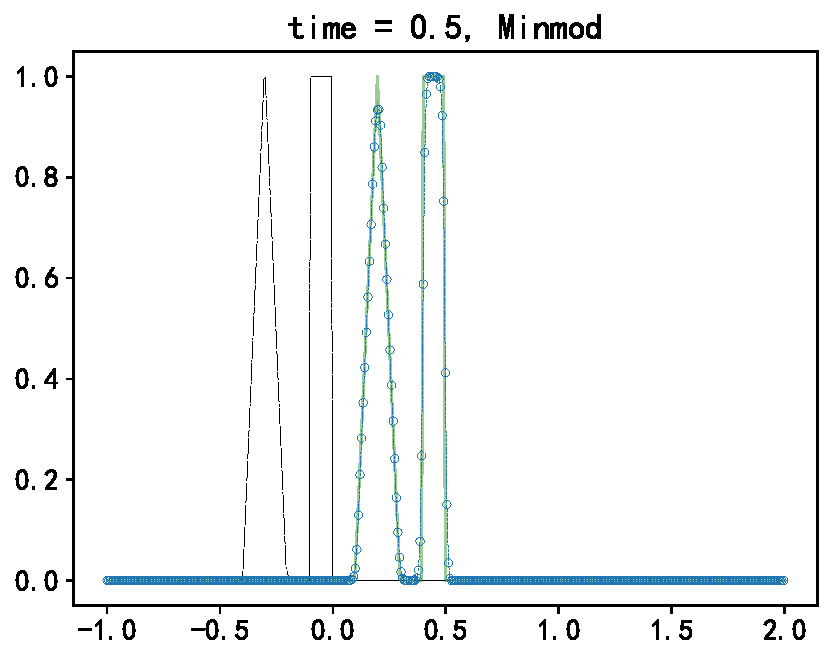
\includegraphics[width=\textwidth]{figures/problem1_limiter0.95.pdf}
  \caption{}
  \label{fig:problem1-6}
\end{subfigure}
\caption{方程~(\ref{EqnCon}) 在 $t=0.5$ 时刻的解. 其中虚线表示数值 \textit{Upwind} 格式的计算结果, 线上的圆圈表示具体网格上的数据. 同一时刻的精确解用实线表示. 作为对照,
  初始时刻的值以点线表示, 坐标网格总数为 517. (a) 迎风格式, $C = 0.05$, (b)  迎风格式, $C = 0.50$, (c)  迎风格式, $C = 0.95$, (d) 迎风格式, $C = 1.0$,
  此时数值解与精确解完全相同, (e) \textit{Lax-Wendroff} 格式, $C = 0.95$,  (f) Minmod格式, $C = 0.95$.} \label{LinearW}
  \label{fig:problem1}%
\end{figure}


数值计算实验采用不同的格式, 不同参数的计算结果.
其中, 实线是精确解, 点线表示初态值, 虚线是数值计算结果, 而圆圈是具体网格 (单元) 上的数据. 

\begin{enumerate}
    \item 比较\textit{Upwind} 格式在网格总数取 428 情况下,
        不同格式, 不同 Courant 系数 ($C = \Delta t / \Delta x$), 在 $t = 0.5$ 的计算结果。
        如图~\ref{LinearW}的前四张所示。可以看到 \textit{Upwind} 格式的数值解在间断处过渡都很平滑。

        其中
\begin{itemize}
	\item $C = 0.05$ 时,$u$随着波的传播被逐渐抹平的情况最为严重,过渡区间宽度最长;
	\item $C = 0.5$ 时, $u$随着波的传播被逐渐抹平;
	\item $C = 0.95$ 时, $u$随着波的传播与精确解几乎一致;
	\item $C = 1.0$ 时数值解与精确解完全一致;
	\item $C = 1.0$ 时,$u$ 的解出现严重振荡,不再像物理解。
\end{itemize}

\item
    比较不同格式,可以看图~\ref{LinearW}的$c$ $e$ $f$三张图。和 \textit{Upwind} 格式相比,其他两种格式的特点如下。
\begin{itemize}
    \item 对于 \textit{Lax-Wendroff} 格式,$C=0.95$ 时, 速度尖峰的高度保持得很好,过渡区间宽度与解析解基本一致,但出现的色散 (上冲和下冲),在间断处出现振荡。
    \item 对于 \textit{Minmod} 格式,三角形速度尖峰高度不如 \textit{Lax-Wendroff} 格式,但比同样是 $C = 0.95$ 的 \textit{Upwind} 格式 (图~\ref{fig:problem1-2} ) 高一些,且方波的形状也保持得更好,过渡区间宽度与解析解基本一致。
\end{itemize}
\end{enumerate}


\subsection{\textit{Burgers}方程数值模拟部分}
考察方程
\begin{align}
\frac{\partial u}{\partial t} + u \frac{\partial u}{\partial x} = 0
\end{align}
在初值为
\begin{align}
u|_{t=0} = \left\{\begin{array}{ll} 1.8, & x < -0.8,
\\
1.4 + 0.4 \cos\left[2 \pi (x + 0.8) \right], & -0.8 \le x < -0.3,
\\
1.0, & -0.3 \le x < 0.0,
\\
1.8, & x \ge 0.0
\end{array} \right.
\end{align}
时的数值解如图~\ref{fig:problem2} 所示。
\begin{figure} 
\centering
\begin{subfigure}{.9\linewidth}
  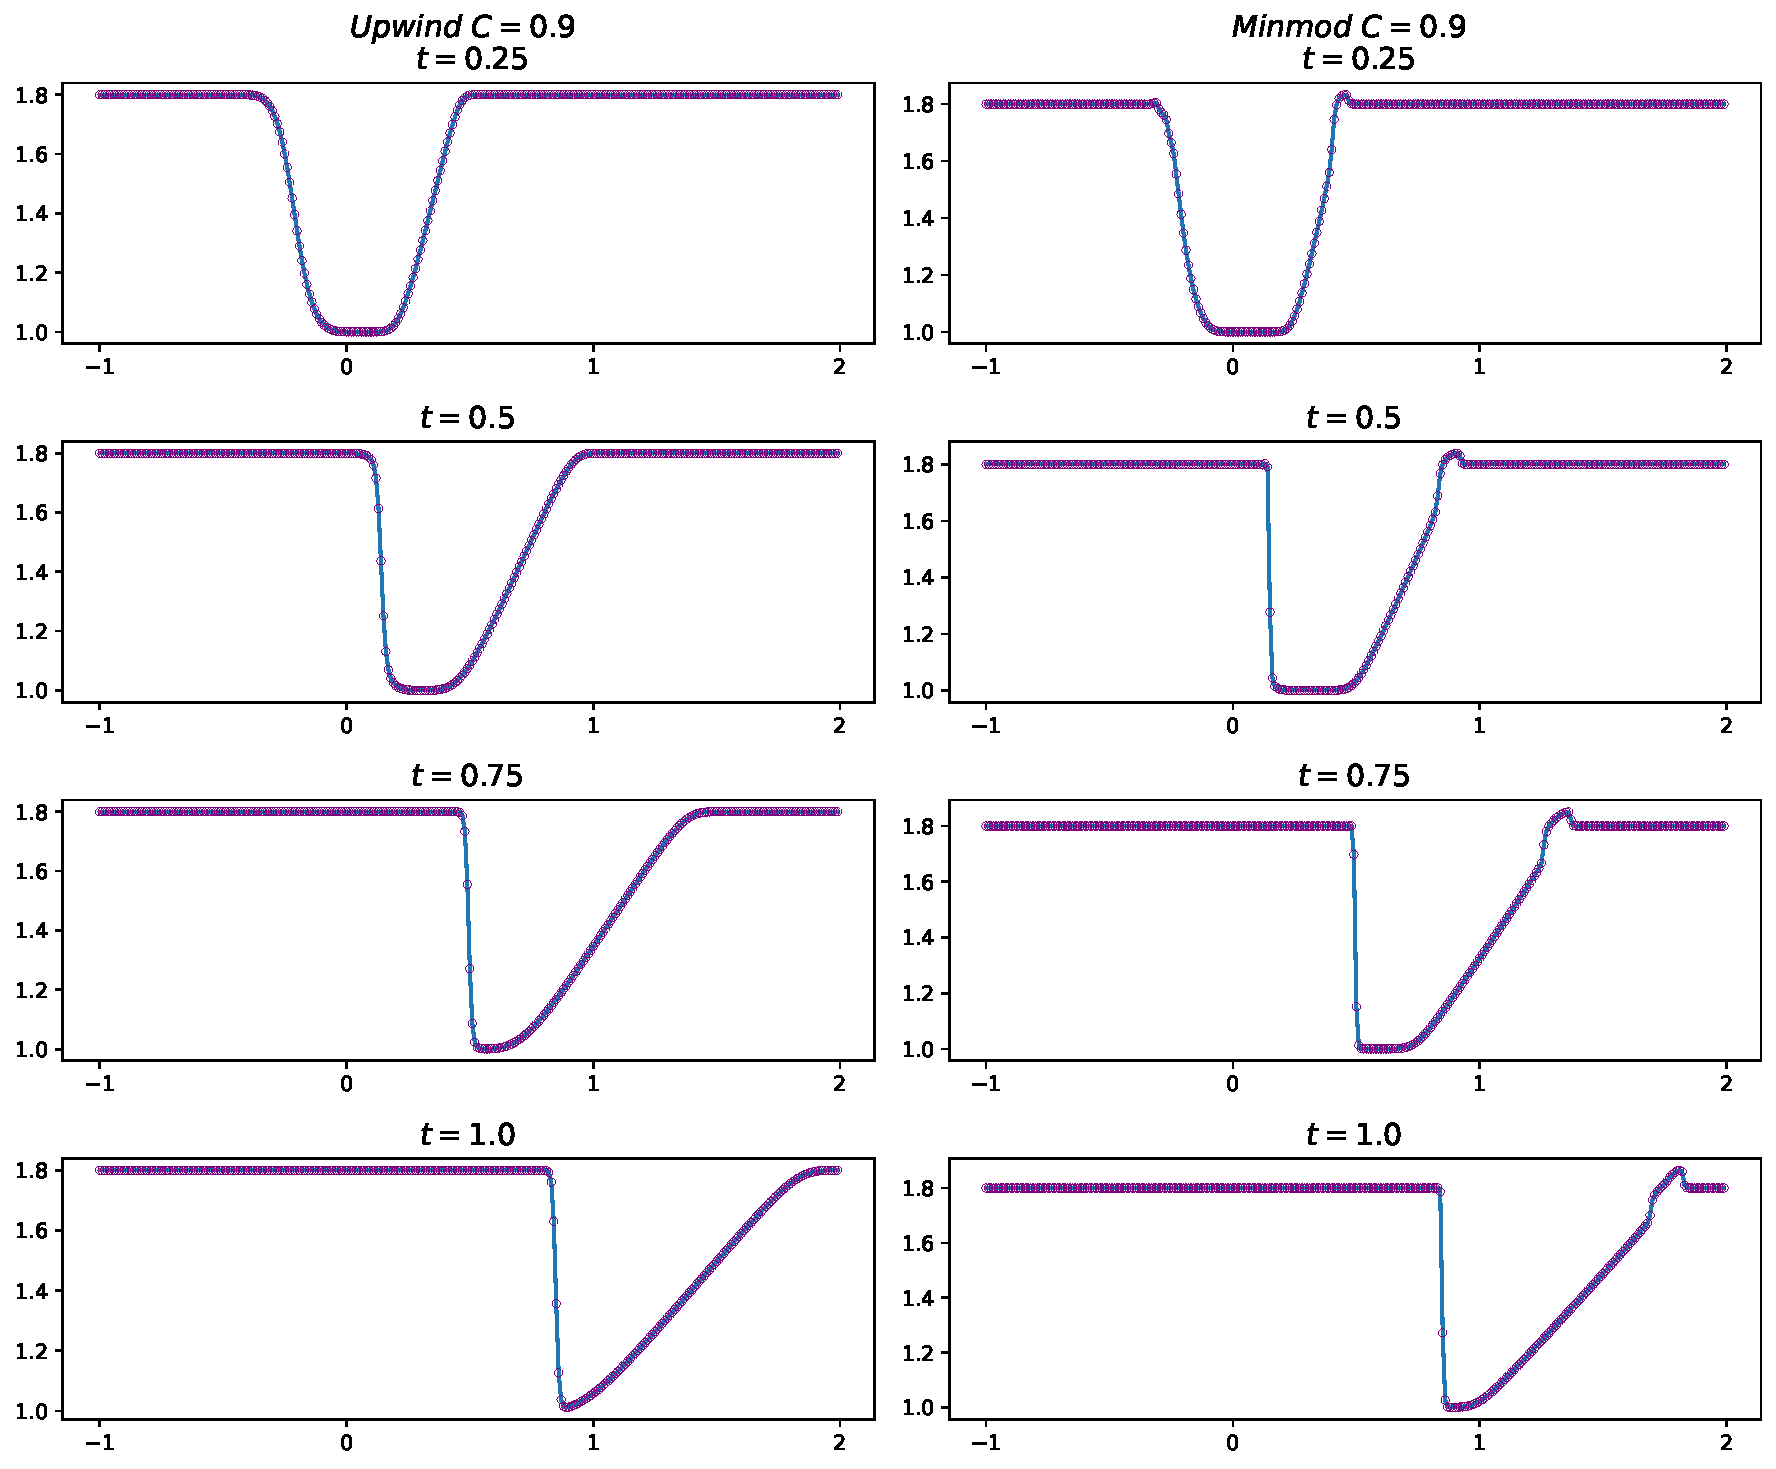
\includegraphics[width=\textwidth]{figures/problem2_myron.pdf} % first figure itself
	\caption{}
  \label{fig:problem2}
\end{subfigure}
\caption{%
    方程~(\ref{EqnBurgers}) 的 \textit{Upwind} 格式与 \textit{Minmod} 格式计算结果, 采用了 100 个网格, 系数 $C  = \Delta t / \Delta = 0.9$. 
    圆圈表示每一个格点的数据;
  从上往下分别取时间为 $t = 0.25$, $t = 0.5$, $t = 0.75$, $t = 1.0$.
}
  \label{fig:problem2}%
\end{figure}

为了能更清晰的对比激波间断以及两种方法的差异色散与耗散,我们将网格间隔稍微调大了一些,用于放大效果。其中每一个小圆圈都代表着一个网格点。
\begin{enumerate}
\item
    纵向来看,波形随着时间向前传播的同时,由于方程自身的特性,
    向上阶跃部分变得平滑,而向下的平滑部分却逐渐形成了激波。
\begin{itemize}
	\item $C = 0.25$ 时,激波尚未形成,但是向上阶跃部分已经趋于平滑;
	\item $C = 0.5$  时,激波基本形成,向前传播;
	\item $C = 0.75$ 时,激波已经形成,继续向前传播;
	\item $C = 1.25$ 时,激波形成,向上阶跃部分已经基本平滑;
\end{itemize}

\item
    横向比较激波效应,可以看到\textit{Upwind} 格式与 \textit{Minmod} 格式的一些特性差异,由于 \textit{Upwind} 格式没有高阶补偿向,
    导致会有持续的耗散,因此激波始终保持着5个左右的间隔距离,
    而 \textit{Minmod} 格式存在高阶补偿项,能够较快速度将激波间隔缩小到2个左右的间隔距离,
    就激波模拟而言 \textit{Minmod} 格式存在一定的优势
\item
    横向比较色散效应,可以看到\textit{Upwind} 格式没有色散只有耗散,而\textit{Minmod} 格式
    存在耗散,具体体现在波前有少量的振荡,同时在原本离散的阶跃处,产生了不应该存在的凸起部分。
\end{enumerate}

\section{分工说明}

代码部分
徐均益写了\verb|main.jl|, 
余航写了\verb|main1.py|、\verb|main2.py|、 \verb|run.sh|。

文档部分
徐均益写了第一部分的线性方程理论与数值解的分析, 余航写了摘要,引言和第二部分非线性方程数值解的分析。
核心公式由徐均益所写。

陈宇韬参与了最后文档校验。
\section{附件}

\begin{enumerate}
\item
main.tex -- 本报告的 \LaTeX 文件
\item
main.pdf -- 本报告的 PDF (Portable Document Format) 输出文件
\item
References.bib -- 文献文件
\item
	\verb|code/main.jl| 本报告的 problem 1 和 problem 2 的 julia 代码
\item
	\verb|code/main.py| 本报告的 problem 1 python 代码
\item
	\verb|code/main2.py| 本报告的 problem 2 python 代码
\item
\verb|figures/problem1_upwind0.05.pdf| -- 行波方程~(\ref{EqnCon}) 的数值计算结果, 对应图~\ref{fig:problem1-1}
\item
\verb|figures/problem1_upwind0.05.pdf| -- 行波方程~(\ref{EqnCon}) 的数值计算结果, 对应图~\ref{fig:problem1-2}
\item
\verb|figures/problem1_upwind0.95.pdf| -- 行波方程~(\ref{EqnCon}) 的数值计算结果, 对应图~\ref{fig:problem1-3}
\item
\verb|figures/problem1_upwind1.0.pdf| -- 行波方程~(\ref{EqnCon}) 的数值计算结果, 对应图~\ref{fig:problem1-4}
\item
\verb|figures/problem1_lax_wendroff0.95.pdf| -- 行波方程~(\ref{EqnCon}) 的数值计算结果, 对应图~\ref{fig:problem1-5}
\item
\verb|figures/problem1_limiter0.95.pdf| - 行波方程~(\ref{EqnCon}) 的数值计算结果, 对应图~\ref{fig:problem1-6}
\item
\verb|figures/problem2_myron.pdf| -- Burgers方程~(\ref{EqnBurgers}) 的数值计算结果, 对应图~\ref{fig:problem2}
\end{enumerate}

\bibliographystyle{apalike}
\bibliography{References}

\end{document}
